\documentclass[12pt]{article}
\usepackage[margin=1in]{geometry}
\usepackage{amsmath}
\usepackage{amsthm}
\usepackage{graphicx}
\usepackage{hyperref}
\usepackage[utf8]{inputenc}
\title{My Statistics 3494W Paper}

\author{Michael  Marcaccio}

\date{September 19 2022}

\begin{document}

\maketitle

\begin{abstract}
  One-paragraph summary of the entire study - typically no more than 250 words in length (and in many cases it is well shorter than that), the Abstract provides an overview of the study.
  \end{abstract}

\section*{Introduction}
\addcontentsline{toc}{section}{Introduction}
What is the Topic and Why is it worth studying? – the first major section of text in the paper, the Introduction commonly describes the topic under investigation, summarizes or discusses relevant prior research (for related details, please see the Writing Literature Reviews section of this website), identifies unresolved issues that the current research will address, and provides an overview of the research that is to be described in greater detail in the sections to follow.



\section*{Methods}
\addcontentsline{toc}{section}{Methods}
What did you do? – a section which details how the research was performed.  It typically features a description of the participants/subjects that were involved, the study design, the materials that were used, and the study procedure.  If there were multiple experiments, then each experiment may require a separate Methods section.  A rule of thumb is that the Methods section should be sufficiently detailed for another researcher to duplicate your research.


\section*{Results}
\addcontentsline{toc}{section}{Results}
What did you find? – a section which describes the data that was collected and the results of any statistical tests that were performed.  It may also be prefaced by a description of the analysis procedure that was used. If there were multiple experiments, then each experiment may require a separate Results section.


\begin{equation}
    \label{eq:area}
    \pi r^2.
\end{equation}


To reference an equation:
Equation~\eqref{eq:area} is about the area of a circle. 
    


An unnumbered equation looks like:
\[
f(x)=\frac{1}{\sqrt{3\pi}}\exp
\]
 
Table~\ref{tab:rv} summarizes some example draws from some distributions.


\begin{table}[ht]
  \caption{This is my first table.}
  \label{tab:rv}
\centering
\begin{tabular}{rrr}
  \hline
normal & poisson & gamma \\ 
  \hline
-0.110 & 4 & 2.401 \\ 
  0.116 & 4 & 3.529 \\ 
  -0.828 & 9 & 2.112 \\ 
  -0.066 & 6 & 11.104 \\ 
  0.219 & 3 & 4.815 \\ 
  0.303 & 5 & 2.188 \\ 
  0.544 & 0 & 8.050 \\ 
  -2.617 & 8 & 3.646 \\ 
  0.747 & 1 & 5.178 \\ 
  -1.103 & 4 & 3.043 \\ 
   \hline
\end{tabular}
\end{table}



Figure~\ref{fig:cars} shows the distance against the speed from this dataset.


\begin{figure}
  \centering
  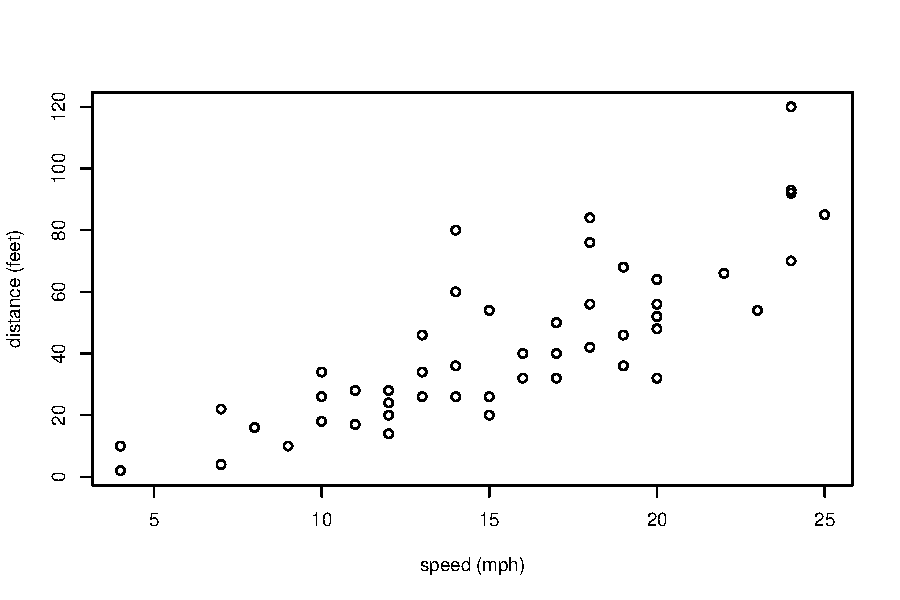
\includegraphics[width=\textwidth]{cars.pdf}
  \caption{This is my first figure.}
  \label{fig:cars}
\end{figure}








\section*{Discussion}
What is the significance of your results? – the final major section of text in the paper.  The Discussion commonly features a summary of the results that were obtained in the study, describes how those results address the topic under investigation and/or the issues that the research was designed to address, and may expand upon the implications of those findings.  Limitations and directions for future research are also commonly addressed.
 

\section*{References}
List of articles and any books cited – an alphabetized list of the sources that are cited in the paper (by last name of the first author of each source).  Each reference should follow specific APA guidelines regarding author names, dates, article titles, journal titles, journal volume numbers, page numbers, book publishers, publisher locations, websites, and so on (for more information, please see the Citing References in APA Style page of this website).







\end{document}
